\chapter{Verdiepend experiment}
De zeezoutbatterij heeft nog geen nautische applicatie. Het is dus niet bekend hoe de batterij reageert op de schommelbewegingen die door de golven worden veroorzaakt. 
\section{Hoofdvraag}
Heeft de dynamica van golven invloed op het vermogen dat de batterij levert?
\section{Opstelling}
Voor dit experiment wordt een zeezoutbatterij (in het rood)  aan één kant van een hefboom (in het bruin) gezet. De andere kant van de hefboom zal handmatig heen en weer bewogen worden met variabele amplitude en frequentie. Op deze manier worden korte golven met hogere frequentie en lange golven met lagere frequentie nagebootst.
\begin{figure}[H]
    \centering
    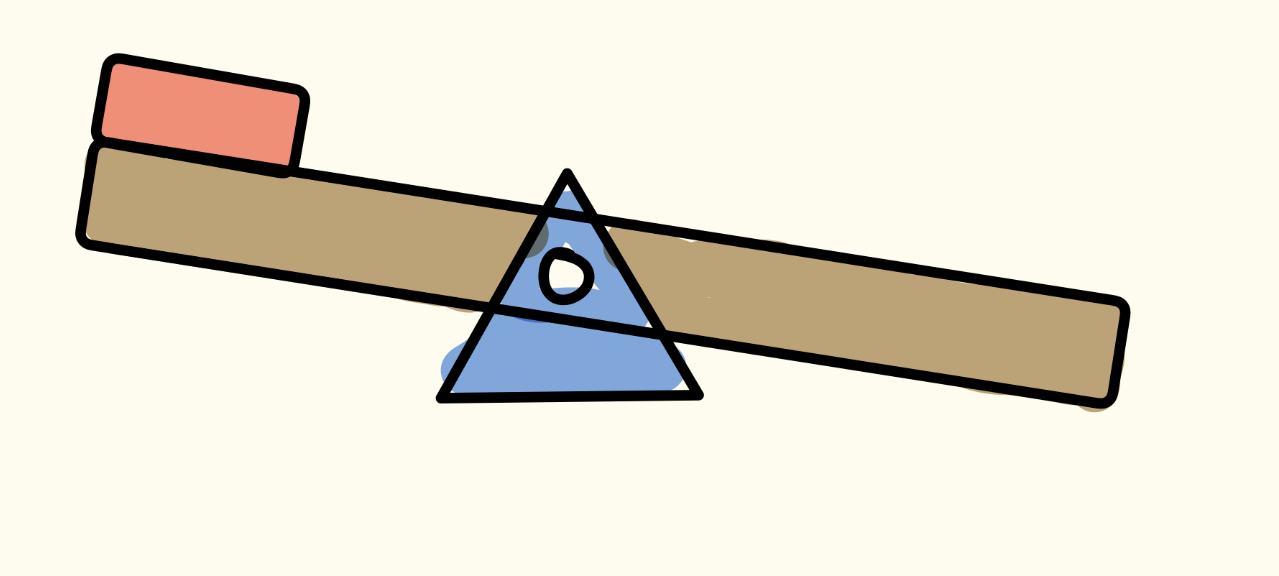
\includegraphics[width=0.5\linewidth]{opstelling.jpeg}
    \caption{Opstelling}
    \label{fig:Opstelling}
\end{figure}

\section{Voorbereiding}
Voor het experiment zijn de volgende onderdelen gebruikt:
\begin{itemize}
    \item \textbf{hefboom}, deze bestaat uit een houten plank met een as daardoorheen
    \item \textbf{multimeter voor stroom}, deze is in serie geschakeld met de batterij.
    \item{\textbf{multimeter voor spanning}, deze is in parallel geschakeld met de batterij en de \textit{load}.
    \item \textbf{\textit{load}}, deze zal bestaan uit een kleine elektromotor, om ervoor te zorgen dat het circuit de stroom ergens kwijt kan.
    \item \textbf{stopwatch} om een constante frequencie aan te houden tijdens de metingen.
\end{itemize}
In Figuur \ref{fig:Circuit} is een schema van de opstelling te zien en in Figuur \ref{fig:fysiek} de daadwerkelijke opstelling.
\begin{figure}[htbp]
    \centering
    \begin{minipage}{0.45\textwidth}
        \centering
        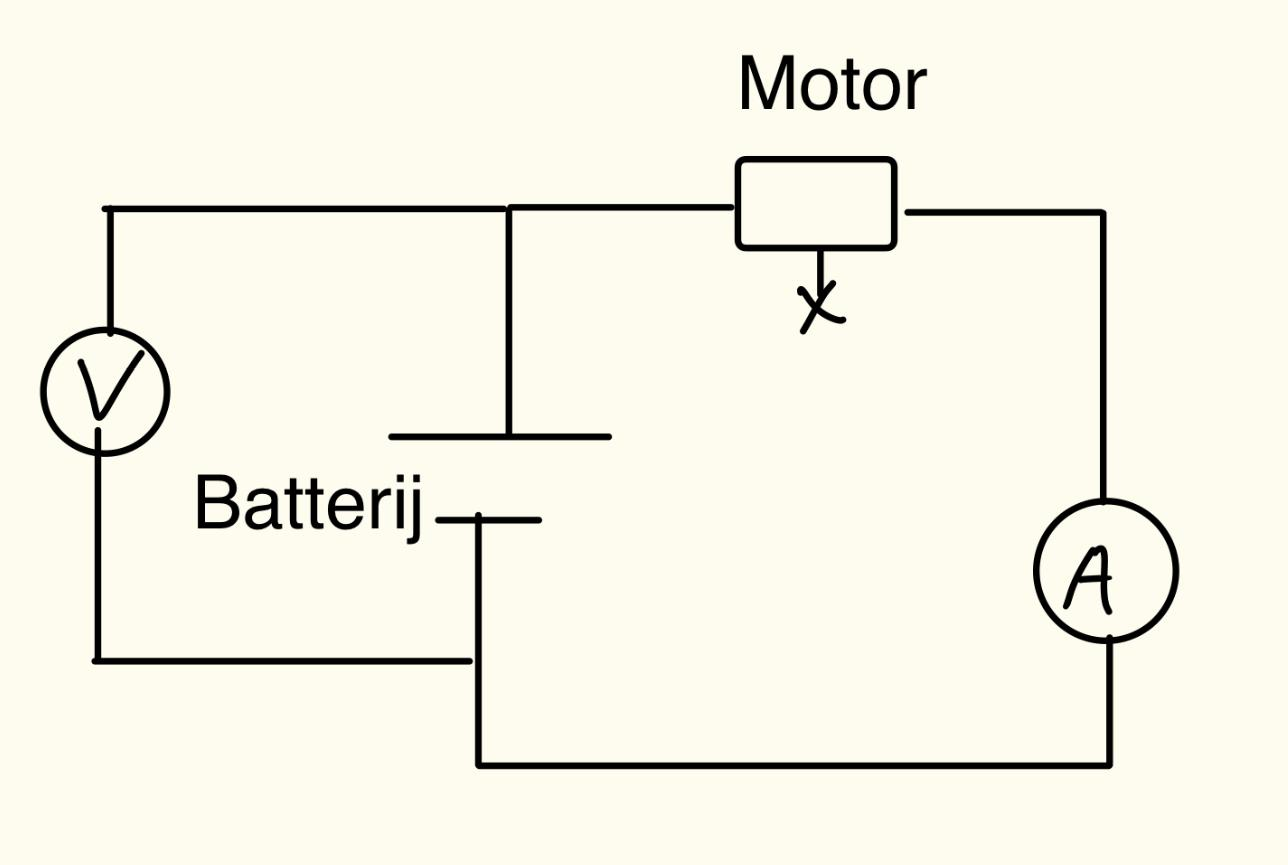
\includegraphics[width=\linewidth]{Circuit.jpeg}
        \caption{Circuit}
        \label{fig:Circuit}
    \end{minipage}\hfill
    \begin{minipage}{0.45\textwidth}
        \centering
        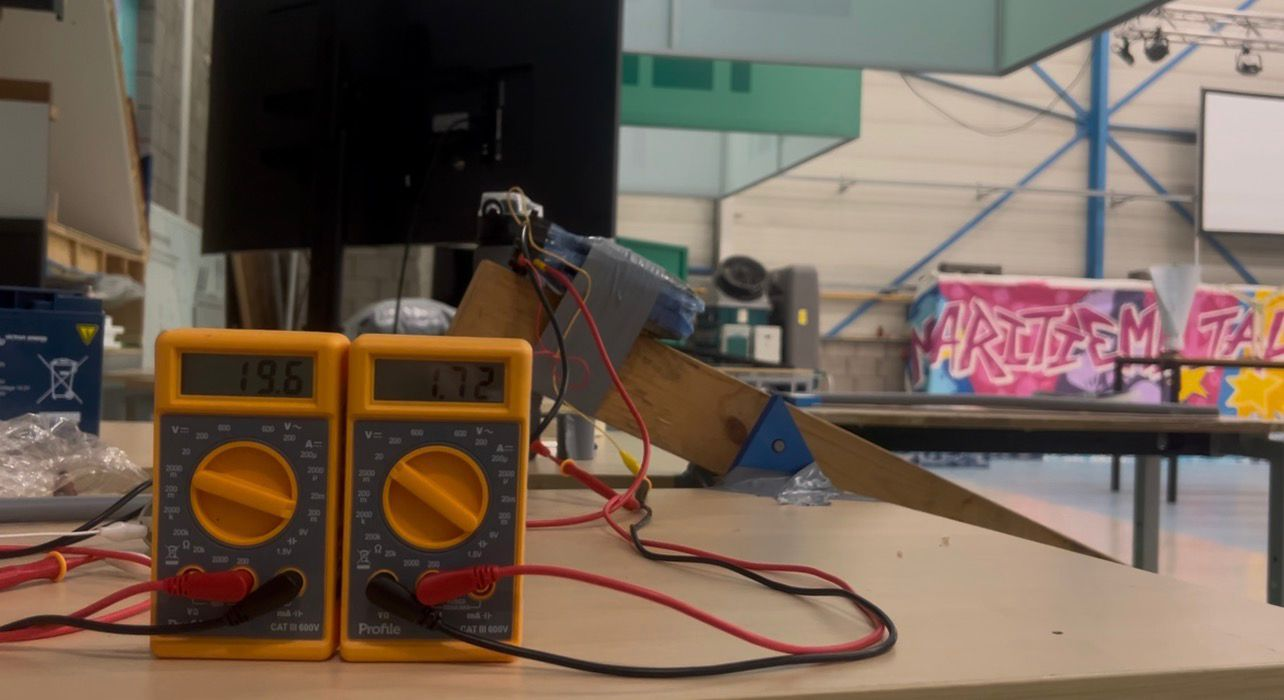
\includegraphics[width=\linewidth]{opstelling].jpeg}
        \caption{Opstelling fysiek}
        \label{fig:fysiek}
    \end{minipage}
\end{figure}

\section{Resultaten}
Met het experiment is de volgende data gerealiseerd:

\begin{table}[htbp]
\centering
\caption{Gemiddelde resultaten onderzoek }
\label{tab:experimental_results}
\begin{tabular}{l c S[table-format=2.3] S[table-format=1.3]}
\toprule
\textbf{Scenario} & \textbf{datapunten} & {\textbf{gemiddelde P (mW)}} & {\textbf{Std afwijking (mW)}} \\
\midrule
*Grote golven      & 60          & 33.664                 & 0.203                     \\
*Kleine golven     & 60          & 33.657                 & 0.172                     \\
\textbf{Statisch 0$^\circ$ (null)} & 60 & \textbf{33.398}     & \textbf{0.197}            \\
Statisch 45$^\circ$ & 59          & 33.442                 & 0.333                     \\
Statisch 90$^\circ$ & 60          & 33.164                 & 0.124                     \\
\bottomrule
\end{tabular}
\end{table}
*Bij de golf scenarios werd een frequentie van circa een trilling per seconde gebruikt, bij lichte golven een hoek van circa 20 graden en bij grote golven circa 45 graden.
\noindent
Deze tabel is een gemiddelde op basis van 60 datapunten met een tijdstap van een seconde, de volledige tabbellen zijn de te vinden in de bijlage [\ref{tab:static_0deg_data}].\\

\noindent
Het vermogen laat een lichte fluctuatie zien, deze fluctuatie is maximaal 0.8 procent van de nulmeting. Te observeren is dat de power afneemt van boven naar beneden in de tabel (bovenste meting is ook de eerste meting en de onderste de laatste meting), de hypothese hiervoor is dat de batterij iets leger is en daardoor (iets) minder krachtig is. 

\section{Conclusie}
Uit bovenstaande resultaten blijkt dat het verschil minder dan een procent is, in absolute termen 0.00026W. Hieruit wordt de conclusie getrokken dat golfbewegingen geen dan wel een verwaarloosbare invloed hebben op de praktische werking van de
batterij in de maritieme omgeving.

\section{Evaluatie}
Om de theorie te valideren dat de batterij leeg raakt en daardoor vermkogen verlies is, zou een volgend experiment gedaan moeten worden waar de batterij tussen sessies door naar het zelfde laadniveau gebracht moeten worden.